% The section about the implemented agents, entities and layers
% @author Kalvin Döge
%


\section{Agententen, Entitäten und Layer}\label{sec:agents-entities-layers}

In diesem Abschnitt wird über das Verhältnis der Agenten, Entitäten und Layer zueinander genauer eingegangen.
Alle Klassen aus der Grafik~\ref{fig:agents-entities-layer} sind gleichbedeutend vom Namen her mit den Komponenten aus dem fachlichen Datenmodell:

\begin{figure}[h]
    \centering
    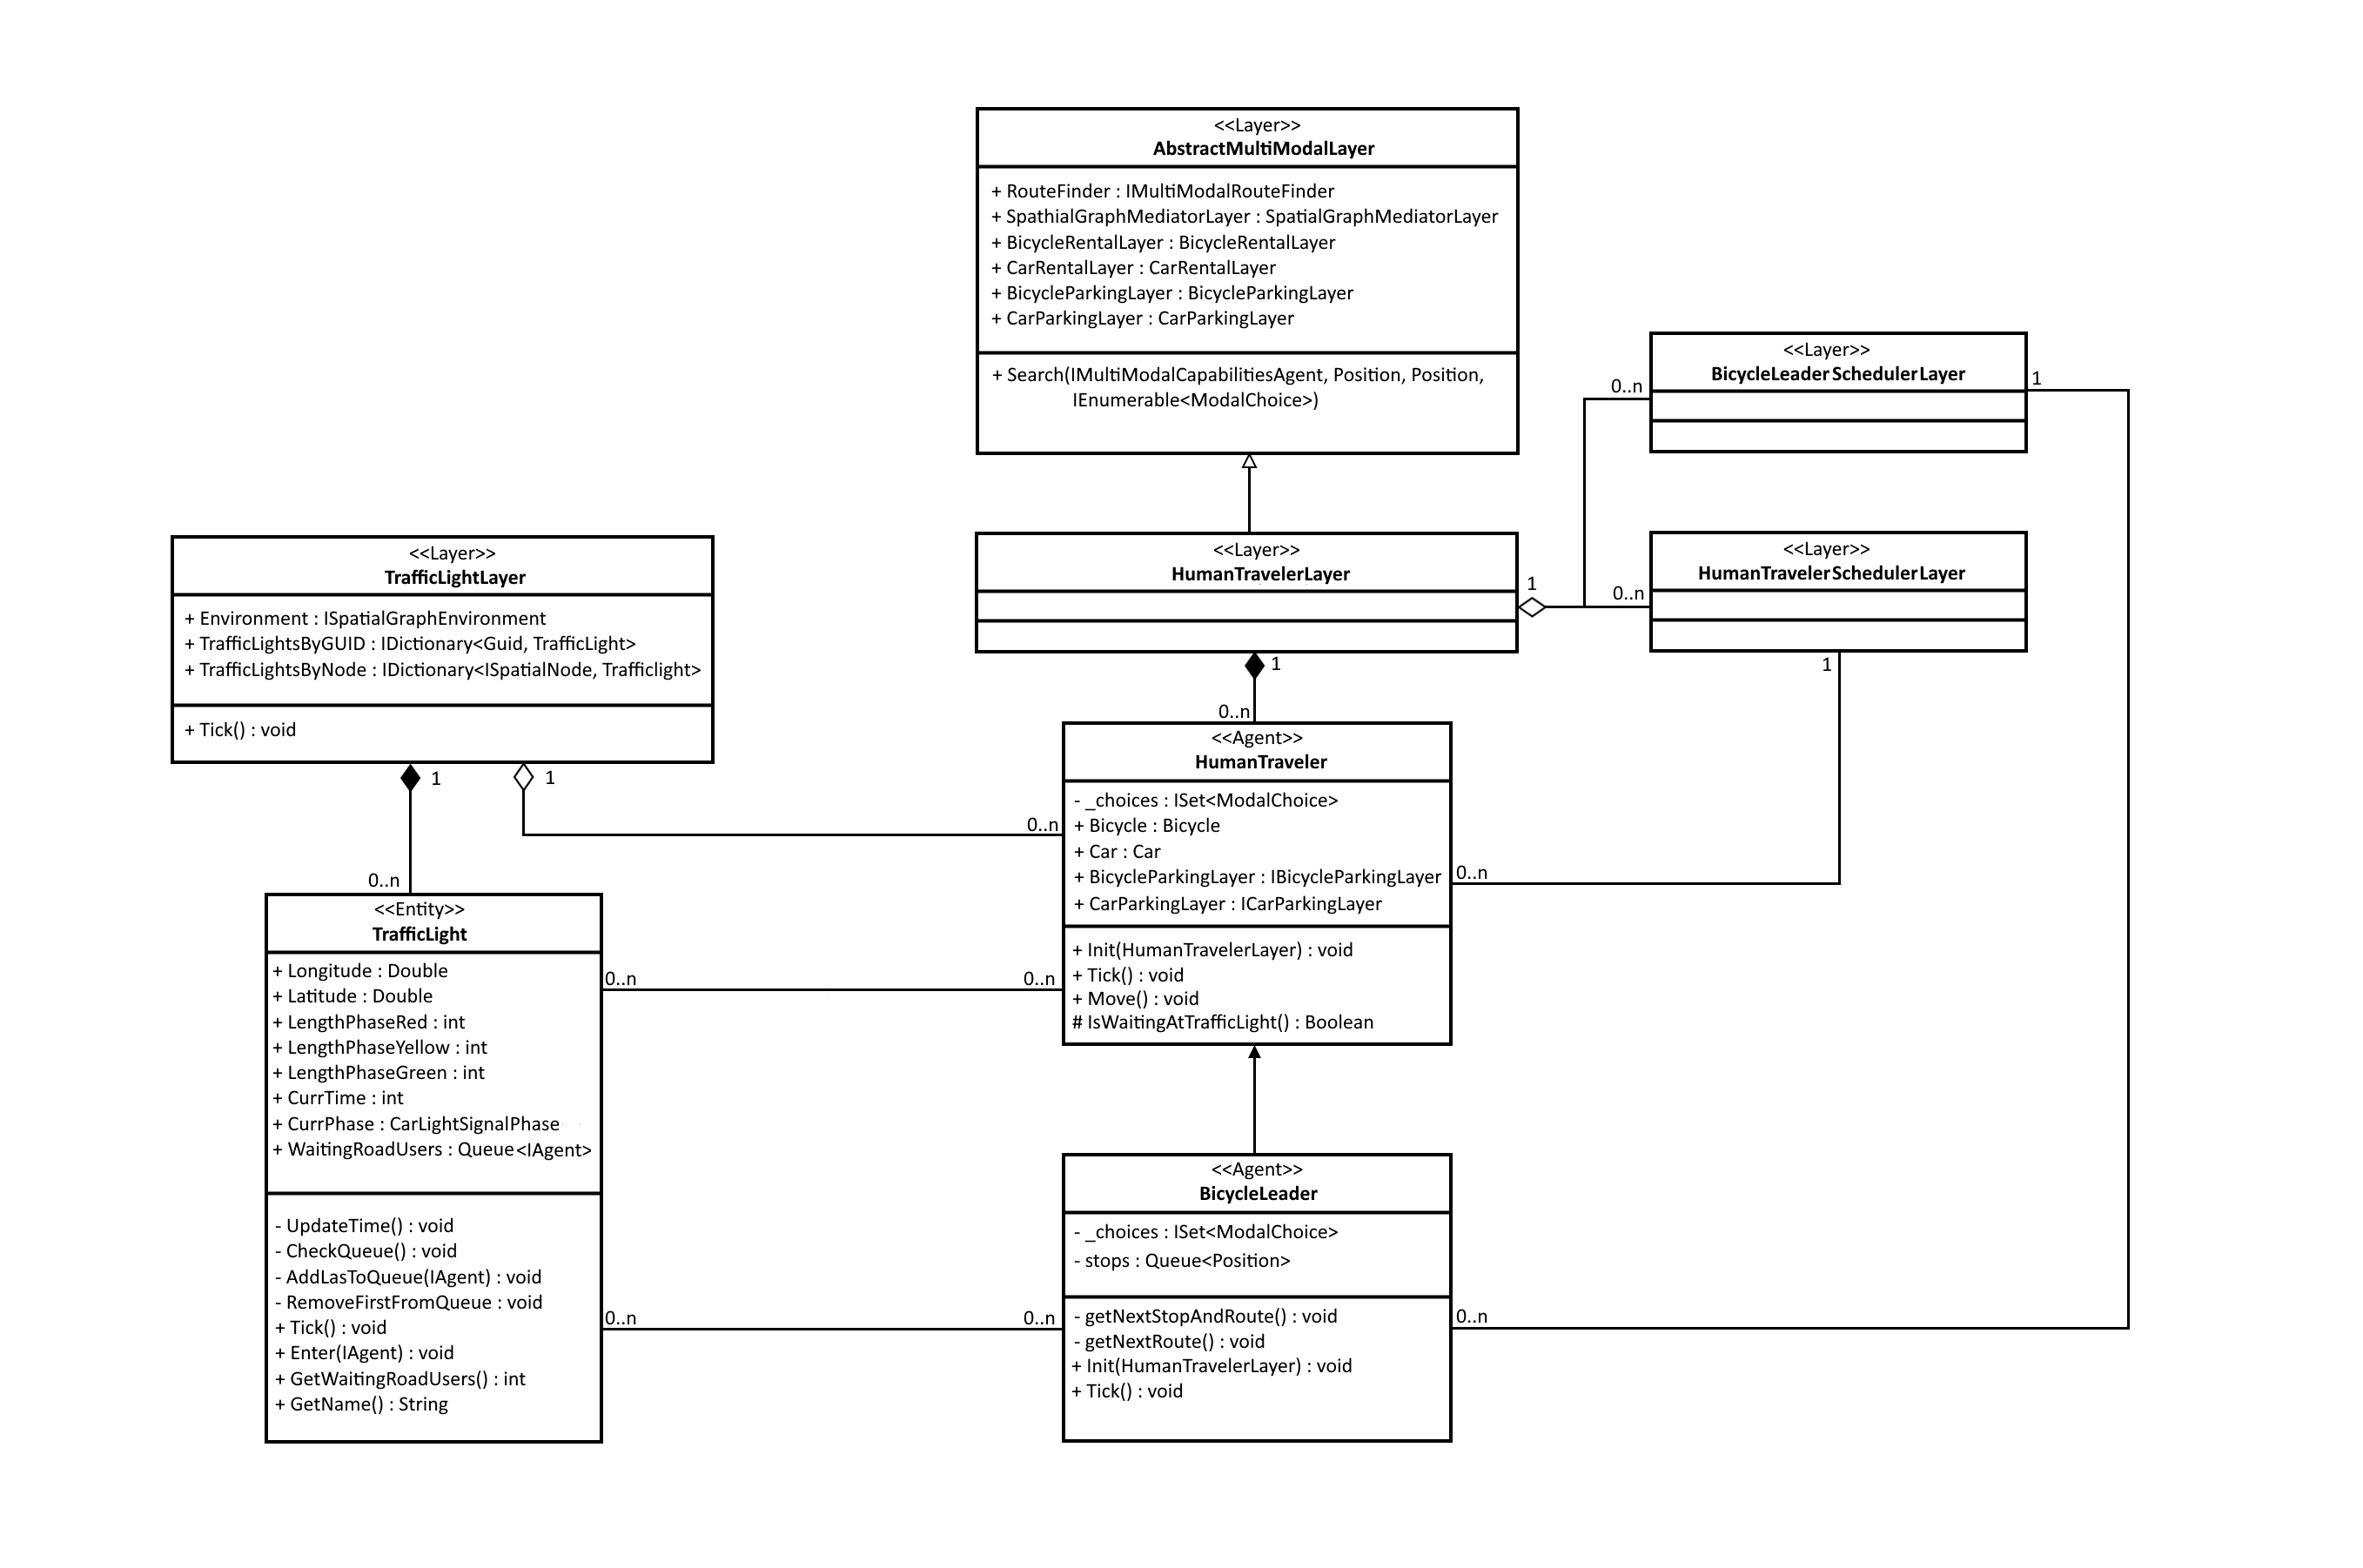
\includegraphics[width=1.00\textwidth]{agents-entities-layer}~\caption{Das technische Datenmodell aller Agenten, Entitäten und Layer}
    \label{fig:agents-entities-layer}
\end{figure}

In der Grafik~\ref{fig:agents-entities-layer} wurden einige überflüssige Eigenschaften, Methoden und Klassen weggelassen, um die Lesbarkeit und Übersichtlichkeit des Datenmodells zu erhöhen.

\textbf{Agent \code{BicycleLeader}:}
\begin{itemize}
    \item Der \code{BicycleLeader} hat Modalitäten zur Auswahl \code{\_choices}, die aber nur das Fahren eines \code{Bicycle}s, \code{RentalBicycle}s und das zu Fuß gehen über \code{WalkingShoes} erlauben.
    \item Dabei ist eine Referenz auf ein \code{Bicycle} und \code{RentalBicycle} gegeben von der geerbten Klasse \code{HumanTraveler}, die wiederum von einer Mehrzahl von Facaden erbt.
    \item Die zu fahrende Route ist beim \code{BicycleLeader} durch die Eigenschaft \code{stops} als Positions-\code{Queue} dargestellt.
    \item \code{BicycleLeader} haben zwei Funktionen zur Verfügung, um den nächsten Schritt ihrer Route zu berechnen: \code{getNextRoute()} sucht mit dem bestehenden Start- und Zielpunkt eine \code{MultimodalRoute}, während die Funktion \code{getNextStopAndRoute()} den nächsten Punkt aus der \code{stops}-Queue entnimmt, dies als das neue Ziel setzt.~Danach wird eine neue Route dorthin berechnet.
    \item Zur Routenberechnung wird der \code{RouteFinder} mit der Methode\linebreak\code{Search(MultiModalCapabilitiesAgent, Position, Position, IEnumerable<ModalChoice>)} aus dem \code{HumanTravelerLayer} aufgerufen.~Die eingegebenen Argumente meinen dabei als erstes den Agenten selbst, also den \code{BicycleLeader}, die Startposition, die Zielposition und die dabei zur Verfügung stehenden Modalitäten des \code{BicycleLeader}s.
    \item Die Funktion \code{Tick()} setzt den nächsten Simulationsschritt des \code{BicycleLeaders} in Gang.~In dieser wird ebenfalls die vom \code{HumanTraveler} geerbte Funktion \code{Move()} ausgeführt.
    \item Die von \code{HumanTraveler} geerbte Funktion \code{IsWaitingAtTrafficLight()} wird ebenso in \code{Tick()} aufgerufen, um auf eine naheliegende \code{TrafficLight} zu prüfen: Ist ihre \code{CurrPhase} entweder \code{CarLightSignalPhase.GREEN}, also grün, oder \code{CarLightSignalPhase.YELLOW}, also gelb, so kann der \code{BicycleLeader} passieren.~Wenn nicht, hält er hier und der \code{BicycleLeader} entfernt sich über einen \code{UnregisterAgent} aus der Simulation.
    \item Hält der \code{BicycleLeader}, so gibt er dies an zusammen mit dem Standort des \code{TrafficLight}s.
\end{itemize}

\textbf{Agent \code{HumanTraveler}:}
\begin{itemize}
    \item Der \code{HumanTraveler} hat alle Modalitäten zur Auswahl: \code{Car}, \code{Bicycle}, \code{RentalCar}, \code{RentalBicycle} und \code{WalkingShoes}.
    \item Die zu fahrende Route ist beim \code{HumanTraveler} durch die Funktion \linebreak\code{Init(HumanTravelerLayer)} gegeben.~Diese ruft die \code{Init(TLayer)}-Funktion der Elternklasse \code{Traveler} auf, in der zwei zufällige Punkte aus der Start- und Zielgeometrie genommen und als Start- und Zielposition festgelegt werden.~Über ein Aufruf der \code{Tick()}-Funktion wird dann die Route berechnet zwischen den Punkten.
    \item \code{HumanTraveler} benutzen ebenfalls die \code{Search(...)}-Funktion des \code{HumanTravelerLayer}s, um die Route berechnen zu lassen.
    \item \code{Tick()} setzt auch beim \code{HumanTraveler} über den Aufruf von \code{Move()} die Bewegung fort.
    \item Der \code{HumanTraveler} prüft ebenfalls mithilfe \code{IsWaitingAtTrafficLight()} vor dem Bewegen, ob er an einer \code{TrafficLight} steht.~Wenn ja, betritt er die Warteschlange von ihr.~Wechselt die \code{TrafficLight} die \code{CurrPhase} zu \code{CarLightSignalPhase.YELLOW} oder \code{CarLightSignalPhase.GREEN}, so fährt er weiter.
\end{itemize}

\textbf{Entität \code{TrafficLight}:}
\begin{itemize}
    \item Die \code{TrafficLight} ist definiert über die Position als \code{Longitude} und \code{Latitude}, eine festgelegte \code{LengthPhaseRed}, \code{LengthPhaseYellow} und \code{LengthPhaseGreen} und hat eine zufällige Zahl zwischen einer dieser Phasen als \code{CurrTime}.~Sie ist zufällig gewählt, damit keine Synchronisation mit den anderen Ampeln vorliegt.
    \item Die \code{WaitingRoadUsers} ist die Warteschlange der wartenden Agenten.
    \item Diese wird durch die \code{CheckQueue()}-Funktion immer wieder überprüft, ob ein Agent aus der Warteschlange entfernt werden kann.~Ist die \code{CurrPhase} bei \code{GREEN} oder \code{YELLOW}, wird pro \code{Tick()}-Aufruf der vorderste der Warteschlange entfernt über die Funktion \code{RemoveFirstFromQueue()}.
    \item \code{UpdateTime()} erhöht \code{CurrTime} bei jedem Aufruf von \code{Tick()} um 1.~Ist die Summe aller drei \code{PhaseLength}s überschritten, so fängt \code{CurrTime} wieder bei 1 an.
    \item Agenten können über die Funktion \code{Enter(IAgent)} der Warteschlange beitreten, sollten sie der \code{TrafficLight} zu Nahe sein.
    \item Der Name des \code{TrafficLight}s setzt sich aus der \code{Longitude} und \code{Latitude} zusammen und wird für die Erkennung genutzt bei der Ausgabe.
\end{itemize}

\textbf{Layer \code{HumanTravelerLayer}:}
\begin{itemize}
    \item Alle \code{HumanTraveler} und \code{BicycleLeader} werden im \code{HumanTravelerLayer} festgehalten und ihre Position über den \code{SpatialGraphMediatorLayer} zusammengefasst.
    \item Der \code{HumanTravelerLayer} implementiert \code{AbstractMultiModalLayer} und stellt damit die verschiedenen Modalitäts-Layer \code{HumanTraveler}n und \code{BicycleLeader}n bereit zum Interagieren.
\end{itemize}

\textbf{Layer \code{TrafficLightLayer}:}
\begin{itemize}
    \item Alle \code{TrafficLight}s werden im \code{TrafficLightLayer} festgehalten über zwei \code{Dictionary}s:
    \begin{itemize}
        \item \code{TrafficLightsByGUID}, wenn eine \code{GUID} vorliegt und mit der die zugehörige \code{TrafficLight} entnommen werden kann
        \item \code{TrafficLightsByNode}, die über einen \code{SpatialNode}, also über \code{Longitude} und \code{Latitude}-Verortung, abgespeichert werden
    \end{itemize}
    \item Die \code{ISpatialNode}s selbst sind in der \code{Environment} vermerkt und sind befüllt mit Eingabedaten bei der Erstellung über die \code{InitLayer(LayerInitData, RegisterAgent, UnregisterAgent)}-Funktion.~Die \code{LayerInitData} stellt dabei die einzelnen Einträge aus der Konfiguration dar.
\end{itemize}

\textbf{Layer \code{BicycleLeaderSchedulerLayer}:}
\begin{itemize}
    \item Dieser \code{Layer} erhält Eingabedaten mit zeitgebunden Einträgen.~Diese Einträge werden dann über die Funktion \code{Schedule(SchedulerEntry)} der Elternklasse \code{AgentSchedulerLayer} hinzugefügt und erstellen den \code{BicycleLeader} mit den eingegebenen Eigenschaften.
    \item Der \code{BicycleLeaderSchedulerLayer} stellt damit das Factory-Pattern dar: Die Funktion \code{Schedule(SchedulerEntry)} wird mit Eingabedaten aufgerufen, um zu einem bestimmten Zeitpunkt einen \code{BicycleLeader} zu erstellen.
\end{itemize}

\textbf{Layer \code{HumanTravelerSchedulerLayer}:}
\begin{itemize}
    \item Identisch zu dem BicycleLeaderSchedulerLayer erhält dieser \code{Layer} Eingabedaten mit zeitgebunden Einträgen.~Diese Einträge werden dann über die Funktion \code{Schedule(SchedulerEntry)} der Elternklasse \code{AgentSchedulerLayer} hinzugefügt und erstellen den \code{HumanTraveler} mit den eingegebenen Eigenschaften.
    \item Der \code{HumanTravelerSchedulerLayer} stellt damit ebenso das Factory-Pattern dar: Er wird mit Eingabedaten aufgerufen, um zu einem bestimmten Zeitpunkt einen \code{HumanTraveler} zu erstellen.
\end{itemize}
